\documentclass[12pt]{article}
\usepackage{fullpage}
\usepackage{amsmath}
\usepackage{amssymb}
\newtheorem{proof}{PROOF}
\usepackage{algorithm}
\usepackage{algpseudocode}
\usepackage{graphicx}
\graphicspath{ {images/} }

\title{Homework 4}
\author{Young Won Kim (yk41) and Minh Pham (mnp7)}
\date{Spring 2017}


\begin{document}
\maketitle
\noindent \textbf{1 Kernelizing k-nearest neighbors} \\
\\ 
Distance between two training examples in K-nearest neighbors 
\\
\\
$\|\phi (x) - \phi (x') \| ^2 = \Sigma (\phi_i (x) - \phi_i (x'))^2$
\\
\\
$\|\phi (x) - \phi (x') \| ^2  = \Sigma (\phi_i(x)^2 - \phi_i(x')^2 - 2\phi_i(x)\phi_i(x')) = k(x,x) - k(x',x') - 2k(x,x')$ \\

KNN algorithms is 3 kernelized functions of $k(x,x), k(x',x')$, and $k(x,x')$.\\
\\
\noindent \textbf{2 Constructing kernels} \\
\\
$k(x,x') = c k_1(x,x')$ for $c > 0$\\
$\alpha^T k \alpha = c \alpha^T k_1 \alpha \geq 0$\\
$k(x,x')$ is positive semi definite and thus, $k(x,x')$ is a valid kernel
\\
\\
$k(x,x') = f(x)k_1(x,x')f(x')$\\
$k(x,x') = f(x)f(x')k_1(x,x')$\\
$k(x,x') = (\psi(x)^T \psi(x')) k_1(x,x')$\\
$k(x,x') = k(\psi(x), \psi(x'))k_1(x,x')$\\
We have, $k(\psi(x), \psi(x')) \geq 0$ and  $k_1(x,x') \geq 0$\\
Therefore, $k(x,x')$ is positive semi definite and thus, $k(x,x')$ is a valid kernel
\\
\\
$k(x,x') = k_1(x,x') + k_2(x,x')$\\
$\alpha^Tk\alpha = \alpha^Tk_1\alpha + \alpha^Tk_2\alpha \geq 0$\\
$k(x,x')$ is positive semi definite and thus, $k(x,x')$ is a valid kernel\\
\\
\\
\noindent \textbf{3 Fitting an SVM classifier by hand} \\
\\$D = {(0,-1),(\sqrt(2),+1)}$ and $\phi(x) = (1, \sqrt(2)x, x^2)$
\\
\\
$min \frac{1}{2} \|\theta\|^2$ \\

s.t. $y^{(1)}(\theta^T\phi(x^{(1)}) + \theta_0) \geq 1$ and $y^{(2)}(\theta^T\phi(x^{(2)}) + \theta_0) \geq 1$\\
\\
Point 1: $(0,-1) \rightarrow (1,0,0)$ and Point 2: $(\sqrt(2), +1) \rightarrow (1,2,3)$ \\
\\
The vector parallel with $\theta$ is $\theta^* = \phi(x_2) - \phi(x_1) = [0, 2, 2]$\\
\\
To solve for margin:\\
$margin = \frac{1}{\|\theta\|} $\\
$\rightarrow \|\theta\| = \frac{1}{\sqrt {2}}$\\
\\
\\To solve for $\theta$:\\
We have, $\theta = k \theta^*$\\
$\rightarrow \sqrt{x_1^2 + x_2^2 + x_3^2} = \sqrt {k^2 (x_{1*}^2 + x_{2*}^2 +x_{3*}^2)} =  \frac{1}{\sqrt{2}}$\\
$\rightarrow k\sqrt{0 + 4 + 4} = \frac{1}{\sqrt(2)} \rightarrow k =  \frac{1}{4}$ \\
\\
Therefore, $\theta = k\theta^* = [0, 0.5, 0.5]$ \\
\\
\\ 
To solve for the intercept $\theta_0$:\\
Since the two points are supporting vectors, the inequalities are tight.\\
$y^{(1)}(\theta^T\phi(x^1) + \theta_0) = -1([0,0.5, 0.5]^T [1,0,0] + \theta_0] = -\theta_0 = 1 $ \\
$y^{(1)}(\theta^T\phi(x^1) + \theta_0) = +1([0,0.5, 0.5]^T [1,2,2] + \theta_0] = 2+ \theta_0 = 1 $ \\
$\rightarrow \theta_0 = -1 $\\
\\
The equation for the decision boundary:\\
$y = \theta^T\phi(x) + \theta_0 = [0, 0.5, 0.5]^T \phi(x) - 1$ where $\phi(x) = (1, \sqrt{2}x, x^2)$\\

	\noindent \textbf{4 Support vector machines for binary classification} \\
	\\
	\noindent \textbf{4.1A The hinge loss function and gradient} \\
	\indent We get: J =  1.0  grad =  [-0.12956186 -0.00167647] \\
	\\
	\noindent \textbf{4.1B Example dataset1: impact of varying C}\\
	\indent When C=1, SVM misclassifies one data point (Figure 1).\\
	\indent When C=100, SVM classifies every point correctly, but the margin is narrower (Figure 2).\\
	\\
	\noindent \textbf{4.1C Gaussian Kernel}\\
	\indent We get Gaussian kernel value of 0.324652467358.\\
	\\
	\noindent \textbf{4.2 Example dataset3: selecting hyperparameters for SVMs}\\
	\indent The hyperparameters that give the best accuracy (=0.96) are sigma= 0.1 c= 0.1. \\
	\indent The decision boundary returned with our best parameters is shown in Figure 3.\\
	
	\begin{figure}[!tpb]
		\centerline{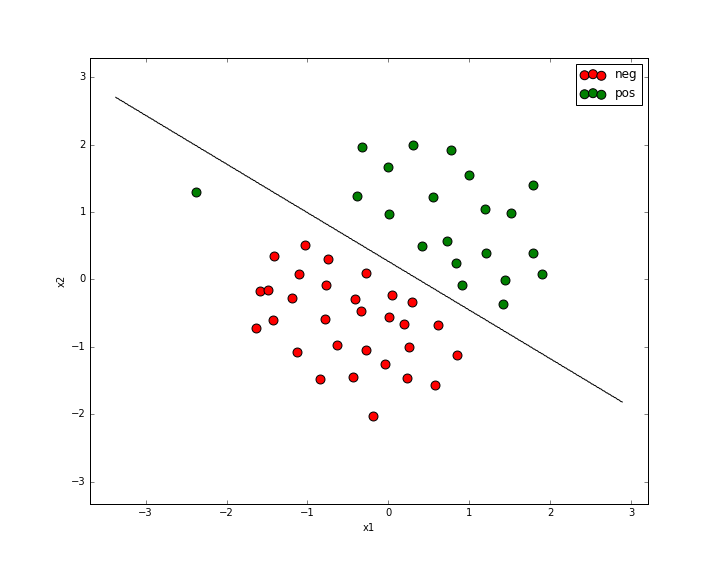
\includegraphics[width=80mm]{decision_boundary_c1.png}}
		\caption{\label{Fig1}
			SVM decision boundary with C=1}
	\end{figure}

	\begin{figure}[!tpb]
		\centerline{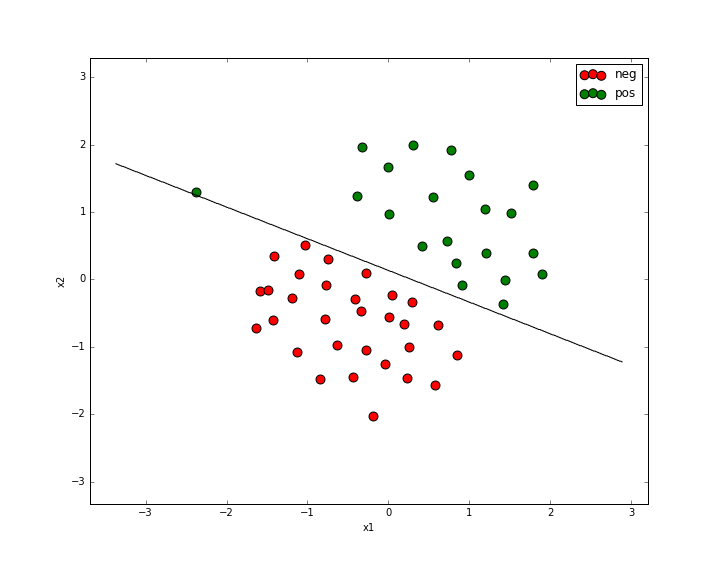
\includegraphics[width=80mm]{decision_boundary_c100.png}}
		\caption{\label{Fig2}
			SVM decision boundary with C=100}
	\end{figure}

	\begin{figure}[!tpb]
		\centerline{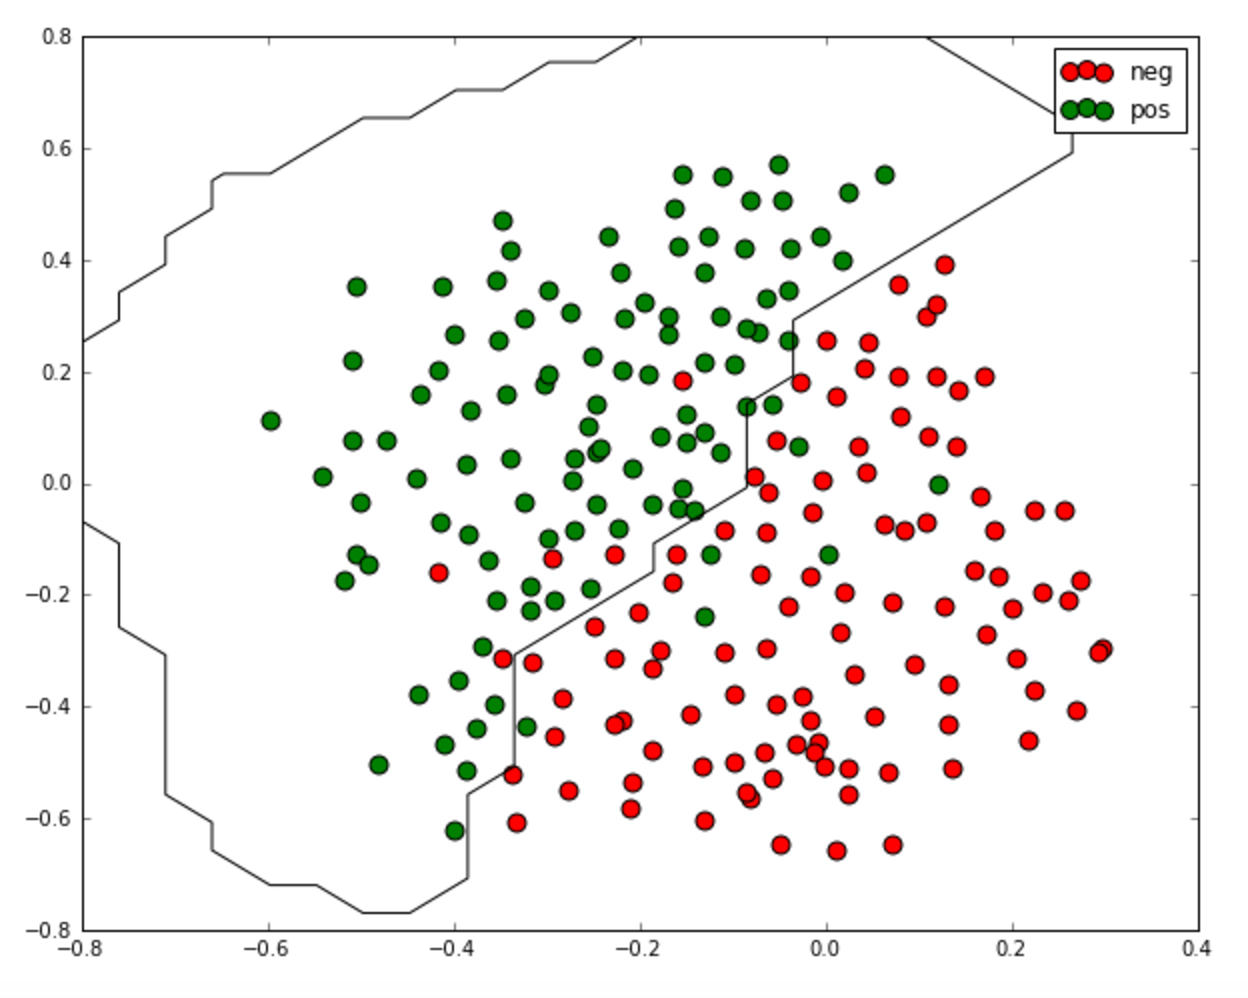
\includegraphics[width=80mm]{SVM_gaussian.png}}
		\caption{\label{Fig3}
			SVM gaussian kernel decision boundary with best hyperparameters}
	\end{figure}
	
	\noindent \textbf{4.3 Spam Classification with SVMs}\\
	(Explain how you chose the parameters for training the SVM, providing graphs and tables to support your choices. Give us your best valus for all of the chosen parameters and hyperparameters. Finally, evaluate the accuracy of your model on the test set and report it.)\\
	learning rate =\\
	number of it = \\
	C = \\
	best kernel = \\
	best hyperparameters for this kernel \\
	
	\noindent \textbf{5 Support vector machines for multi-classification}
	
	SVM takes longer to train and achieves lower performance. Best accuracy for SVM was 0.393, whereas best accuracy for Softmax was 0.411. The visualizations of parameters learned by both methods look very similar. Best hyperparamers for SVM were lr=5.0e-07 and reg=1.0e+04, and best hyperparameters for Softmax were lr=1.0e-06 and reg=5.0e+04. 
	
	
	
	\begin{figure}[!tpb]
		\centerline{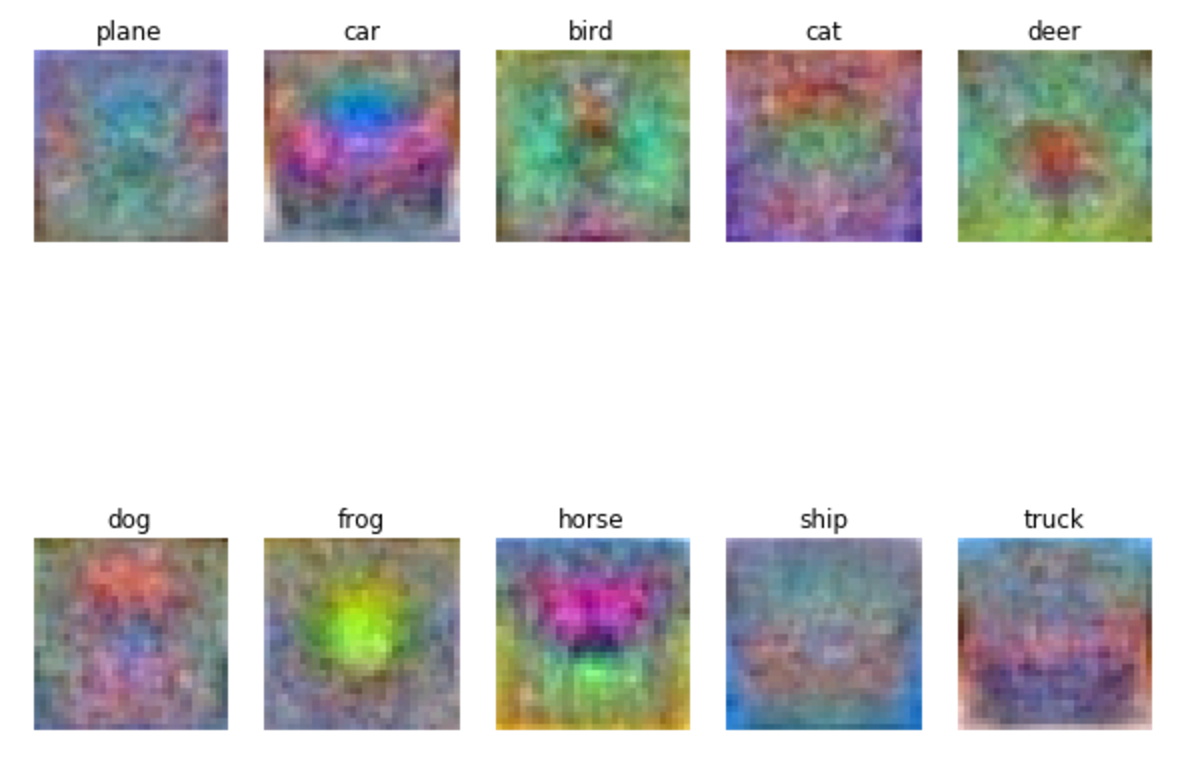
\includegraphics[width=80mm]{best_svm.png}}
		\caption{\label{Fig4}
			Visualization - SVM}
	\end{figure}
	
	\begin{figure}[!tpb]
		\centerline{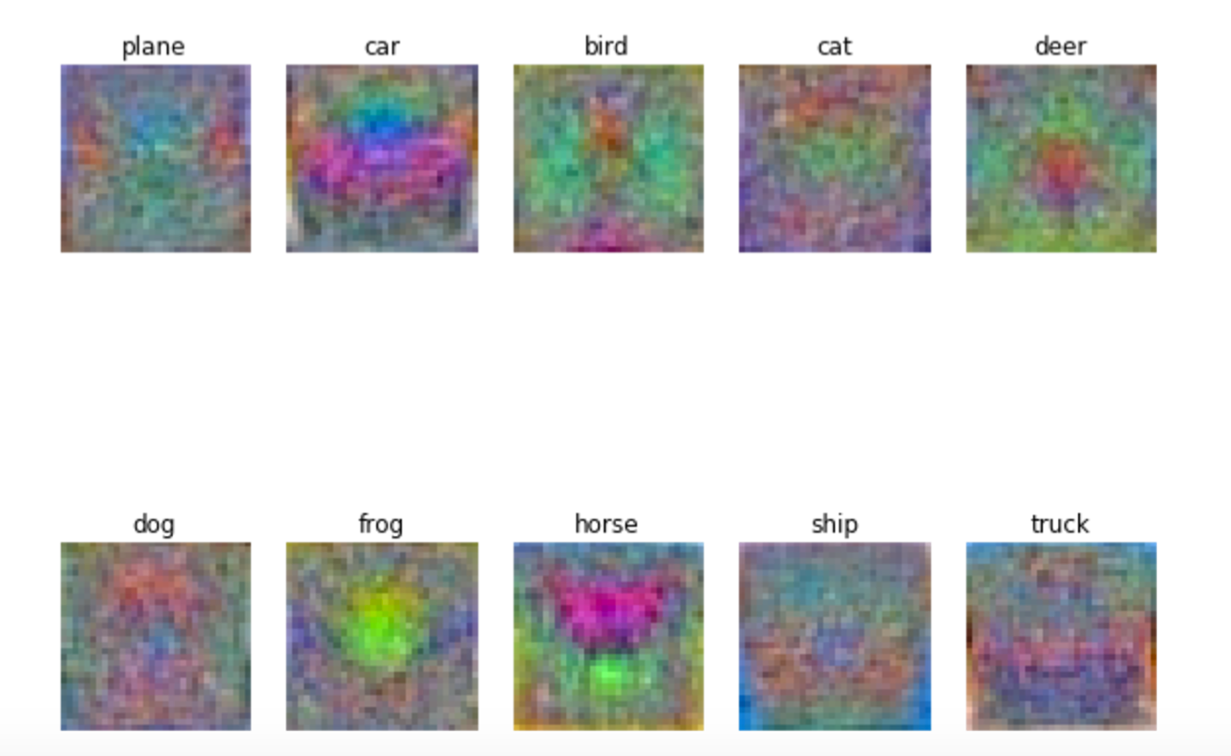
\includegraphics[width=80mm]{CIFAR-10.png}}
		\caption{\label{Fig5}
			Visualization - Softmax}
	\end{figure}

\end{document}